% generated by GAPDoc2LaTeX from XML source (Frank Luebeck)
\documentclass[a4paper,11pt]{report}

\usepackage{a4wide}
\sloppy
\pagestyle{myheadings}
\usepackage{amssymb}
\usepackage[utf8]{inputenc}
\usepackage{makeidx}
\makeindex
\usepackage{color}
\definecolor{FireBrick}{rgb}{0.5812,0.0074,0.0083}
\definecolor{RoyalBlue}{rgb}{0.0236,0.0894,0.6179}
\definecolor{RoyalGreen}{rgb}{0.0236,0.6179,0.0894}
\definecolor{RoyalRed}{rgb}{0.6179,0.0236,0.0894}
\definecolor{LightBlue}{rgb}{0.8544,0.9511,1.0000}
\definecolor{Black}{rgb}{0.0,0.0,0.0}

\definecolor{linkColor}{rgb}{0.0,0.0,0.554}
\definecolor{citeColor}{rgb}{0.0,0.0,0.554}
\definecolor{fileColor}{rgb}{0.0,0.0,0.554}
\definecolor{urlColor}{rgb}{0.0,0.0,0.554}
\definecolor{promptColor}{rgb}{0.0,0.0,0.589}
\definecolor{brkpromptColor}{rgb}{0.589,0.0,0.0}
\definecolor{gapinputColor}{rgb}{0.589,0.0,0.0}
\definecolor{gapoutputColor}{rgb}{0.0,0.0,0.0}

%%  for a long time these were red and blue by default,
%%  now black, but keep variables to overwrite
\definecolor{FuncColor}{rgb}{0.0,0.0,0.0}
%% strange name because of pdflatex bug:
\definecolor{Chapter }{rgb}{0.0,0.0,0.0}
\definecolor{DarkOlive}{rgb}{0.1047,0.2412,0.0064}


\usepackage{fancyvrb}

\usepackage{mathptmx,helvet}
\usepackage[T1]{fontenc}
\usepackage{textcomp}


\usepackage[
            pdftex=true,
            bookmarks=true,        
            a4paper=true,
            pdftitle={Written with GAPDoc},
            pdfcreator={LaTeX with hyperref package / GAPDoc},
            colorlinks=true,
            backref=page,
            breaklinks=true,
            linkcolor=linkColor,
            citecolor=citeColor,
            filecolor=fileColor,
            urlcolor=urlColor,
            pdfpagemode={UseNone}, 
           ]{hyperref}

\newcommand{\maintitlesize}{\fontsize{50}{55}\selectfont}

% write page numbers to a .pnr log file for online help
\newwrite\pagenrlog
\immediate\openout\pagenrlog =\jobname.pnr
\immediate\write\pagenrlog{PAGENRS := [}
\newcommand{\logpage}[1]{\protect\write\pagenrlog{#1, \thepage,}}
%% were never documented, give conflicts with some additional packages

\newcommand{\GAP}{\textsf{GAP}}

%% nicer description environments, allows long labels
\usepackage{enumitem}
\setdescription{style=nextline}

%% depth of toc
\setcounter{tocdepth}{1}



\usepackage{graphics}
\usepackage{psfrag}
\psfrag{C2}{$C_2$}


%% command for ColorPrompt style examples
\newcommand{\gapprompt}[1]{\color{promptColor}{\bfseries #1}}
\newcommand{\gapbrkprompt}[1]{\color{brkpromptColor}{\bfseries #1}}
\newcommand{\gapinput}[1]{\color{gapinputColor}{#1}}


\begin{document}

\logpage{[ 0, 0, 0 ]}
\begin{titlepage}
\mbox{}\vfill

\begin{center}{\maintitlesize \textbf{The \textsf{SCO} Package Manual\mbox{}}}\\
\vfill

\hypersetup{pdftitle=The \textsf{SCO} Package Manual}
\markright{\scriptsize \mbox{}\hfill The \textsf{SCO} Package Manual \hfill\mbox{}}
{\Huge \textbf{Simplicial Cohomology of Orbifolds\mbox{}}}\\
\vfill

{\Huge  Version 2011.08.11 \mbox{}}\\[1cm]
{August 2011\mbox{}}\\[1cm]
\mbox{}\\[2cm]
{\Large \textbf{Simon G{\"o}rtzen\\
    \mbox{}}}\\
\hypersetup{pdfauthor=Simon G{\"o}rtzen\\
    }
\end{center}\vfill

\mbox{}\\
{\mbox{}\\
\small \noindent \textbf{Simon G{\"o}rtzen\\
    }  Email: \href{mailto://simon.goertzen@rwth-aachen.de} {\texttt{simon.goertzen@rwth-aachen.de}}\\
  Homepage: \href{http://wwwb.math.rwth-aachen.de/goertzen/} {\texttt{http://wwwb.math.rwth-aachen.de/goertzen/}}\\
  Address: \begin{minipage}[t]{8cm}\noindent
 Lehrstuhl B f{\"u}r Mathematik\\
 RWTH Aachen\\
 Templergraben 64\\
 52062 Aachen\\
 (Germany)\\
 \end{minipage}
}\\
\end{titlepage}

\newpage\setcounter{page}{2}
{\small 
\section*{Abstract}
\logpage{[ 0, 0, 2 ]}
This document explains the primary uses of the \textsf{SCO} package. Included in this manual is a documented list of the most important
methods and functions you will need. For the theoretical basis of this package
please refer to my diploma thesis and the corresponding paper (work in
progress; \cite{Goe}). \mbox{}}\\[1cm]
{\small 
\section*{Copyright}
\logpage{[ 0, 0, 1 ]}
 {\copyright} 2007-2011 by Simon G{\"o}rtzen

 This package may be distributed under the terms and conditions of the GNU
Public License Version 2. \mbox{}}\\[1cm]
{\small 
\section*{Acknowledgements}
\logpage{[ 0, 0, 3 ]}
The \textsf{SCO} package would not have been possible without the theoretical work by I.
Moerdijk and D. A. Pronk concerning simplicial cohomology of orbifolds \cite{MP_SCO}. Many thanks to these two, as well as Mohamed Barakat and the Lehrstuhl B
f{\"u}r Mathematik at RWTH Aachen University in general. It should be noted
that \textsf{SCO} in its current functionality is dependent on the \textsf{GAP} package \textsf{homalg} by M. Barakat \cite{homalg}, as it relies on \textsf{homalg} to do the actual computations. This manual was created with the help of the \textsf{GAPDoc} package by M. Neunh{\"o}ffer and F. L{\"u}beck. \mbox{}}\\[1cm]
\newpage

\def\contentsname{Contents\logpage{[ 0, 0, 4 ]}}

\tableofcontents
\newpage

 \index{\textsf{SCO}}   
\chapter{\textcolor{Chapter }{Introduction}}\label{intro}
\logpage{[ 1, 0, 0 ]}
\hyperdef{L}{X7DFB63A97E67C0A1}{}
{
  
\section{\textcolor{Chapter }{Overview over this manual}}\label{overview}
\logpage{[ 1, 1, 0 ]}
\hyperdef{L}{X786BACDB82918A65}{}
{
  Chapter \ref{intro} is concerned with the technical details of installing and running this
package. The following chapter \ref{usage} explains how to use \textsf{SCO} to compute simplicial (co-)homology of orbifolds. For the theoretical parts
please refer to my diploma thesis and the corresponding paper (work in
progress; \cite{Goe}). After this chapter you will find some simple examples on using \textsf{SCO} with (finite) groups, manifolds, or some easy orbifolds. Also included in this
manual is a documented list of the most important methods and functions you
will need to work with \textsf{SCO}'s data types OrbifoldTriangulation and SimplicialSet and to create the
matrices needed for computations. Anyone interested in source code should just
check out the files in the \texttt{gap/pkg/SCO/gap/} folder ($\to$ Appendix \ref{FileOverview}). }

   
\section{\textcolor{Chapter }{Installation of the \textsf{SCO} Package}}\label{install}
\logpage{[ 1, 2, 0 ]}
\hyperdef{L}{X78789F1B80457028}{}
{
  To install this package just extract the package's archive file to the GAP \texttt{pkg/} directory. By default the \textsf{SCO} package is not automatically loaded by \textsf{GAP} when it is installed. You must load the package with \texttt{LoadPackage("SCO");} before its functions become available. Please, send me an e-mail if you have
any questions, remarks, suggestions, etc. concerning \textsf{SCO}. Also, I would like to hear about applications of this package.\\
 Simon Goertzen\\
 }

 }

   
\chapter{\textcolor{Chapter }{Usage}}\label{usage}
\logpage{[ 2, 0, 0 ]}
\hyperdef{L}{X86A9B6F87E619FFF}{}
{
 There are different ways to use \textsf{SCO}. Please note that for the actual computations the \textsf{homalg} package is required, and you will need both the \textsf{RingsForHomalg} and the \textsf{GaussForHomalg} package to make use of the full computational capabilities. For your
information, \textsf{RingsForHomalg} offers support for external computer algebra systems and the rings they
support, while \textsf{GaussForHomalg} extends \textsf{GAP} functionality with regards to sparse matrices and computations over fields and ${\ensuremath{\mathbb Z}} / \langle p^n \rangle$. 

 
\section{\textcolor{Chapter }{The Examples Script}}\label{script}
\logpage{[ 2, 1, 0 ]}
\hyperdef{L}{X79F33723829E90DB}{}
{
 Regardless of the extend of your installation, you will always be able to call
the example script \texttt{SCO/examples/examples.g}. This script is not only callable in-\textsf{GAP} by \texttt{SCO{\textunderscore}Examples} (\ref{SCOExamples}), but also automatically checks which packages you have installed and provides
you with the available options. The example script is designed to take you
through the ring creation process and then load one of the files of your
choice located in the \texttt{SCO/examples/orbifolds/} directory. In there you will find a lot of test files with small 0- or
1-dimensional orbifolds, but also the complete triangulations of the 17
orbifolds corresponding to the 2-dimensional wallpaper groups (these should be
exactly the uncapitalized files, ranging from \texttt{p1.g} to \texttt{p6m.g}). Computing the cohomology of these orbifolds was an important part of my
diploma thesis \cite{Goe} and I have also created a separate document \cite{WGC} to present my results.

 Please note that the variables \mbox{\texttt{\mdseries\slshape M}}, \mbox{\texttt{\mdseries\slshape iso}}, and \mbox{\texttt{\mdseries\slshape mu}} in the orbifold files have to keep their name for the example script to work
correctly. Refer to chapter \ref{examples} for concrete examples. }

 
\section{\textcolor{Chapter }{Working Manually}}\label{manual}
\logpage{[ 2, 2, 0 ]}
\hyperdef{L}{X7F193D117BD03FE3}{}
{
 Once you are familiar with the example script and want to try out your own
triangulations, it is best to create your own \texttt{.g} file in the \texttt{SCO/examples/orbifolds/} directory, then call the script again. If for any reason you do not want to
create a file or work with the script, you can always do every step by hand.
Check \ref{ch:MandF} if you need to know more about specific methods and functions. The basic steps
are:

 
\begin{itemize}
\item Define a list of maximum simplices
\item If applicable, define an isotropy record
\item If applicable, define a list encoding the $\mu$-map
\item From the above data, create an orbifold triangulation
\item Define the simplicial set of the orbifold triangulation
\item Create a \textsf{homalg} ring $R$
\item Create boundary or coboundary matrices over $R$
\item Calculate their homology or cohomology
\end{itemize}
 }

 }

   
\chapter{\textcolor{Chapter }{Examples}}\label{examples}
\logpage{[ 3, 0, 0 ]}
\hyperdef{L}{X7A489A5D79DA9E5C}{}
{
 Although there are some small examples embedded in chapter \ref{ch:MandF}, we will give some complete examples in this chapter. Most of these could
easily be called with the example script mentioned in chapter \ref{usage}, but we will do them step by step for best reproducability. 
\section{\textcolor{Chapter }{Example 1: Klein Bottle}}\logpage{[ 3, 1, 0 ]}
\hyperdef{L}{X8274E5BE843F2E82}{}
{
 Suppose we want to calculate the cohomology of the Klein Bottle. First, we
need a triangulation. It could look like this:  \begin{figure}[htbp] \begin{center} 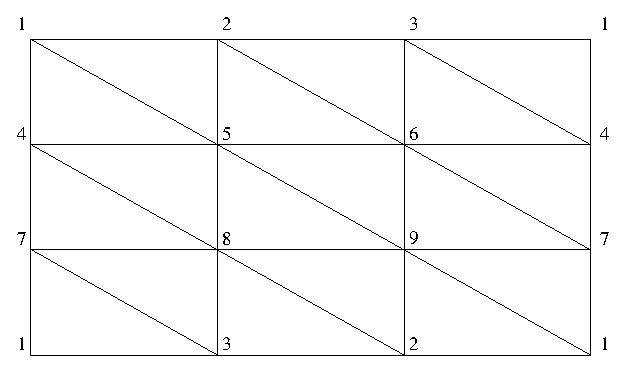
\includegraphics{files/pgt}
\caption{triangulation} \end{center} \end{figure}   

 This results in the following list of maximum simplices: 
\begin{Verbatim}[commandchars=!@|,fontsize=\small,frame=single,label=Example]
  !gapprompt@gap>| !gapinput@M := [ [1,2,4], [1,2,7], [1,3,6], [1,3,8], [1,4,6], [1,7,8],|
  !gapprompt@>| !gapinput@[2,3,5], [2,3,9], [2,4,5], [2,7,9], [3,5,6], [3,8,9],|
  !gapprompt@>| !gapinput@[4,5,7], [4,6,9], [4,7,9], [5,6,8], [5,7,8], [6,8,9] ];;|
\end{Verbatim}
 As there is no isotropy and therefore no $\mu$-map, we can continue with the orbifold triangulation and simplicial set: 
\begin{Verbatim}[commandchars=!@|,fontsize=\small,frame=single,label=Example]
  !gapprompt@gap>| !gapinput@ot := OrbifoldTriangulation( M, "Klein Bottle" );|
  <OrbifoldTriangulation "Klein Bottle" of dimension 2. 18 simplices on 9 vertic\
  es without Isotropy>
  !gapprompt@gap>| !gapinput@ss := SimplicialSet( ot );|
  <The simplicial set of the orbifold triangulation "Klein Bottle", computed up \
  to dimension 0 with Length vector [ 18 ]>
\end{Verbatim}
 Now we will need a \textsf{homalg} ring. As this is a small example we can compute directly over
{\ensuremath{\mathbb Z}}, so we can use \textsf{GAP}. In case you have \textsf{RingsForHomalg} installed you might want to try computing in another computer algebra system
with the command \texttt{HomalgRingOfIntegersInCAS()}, replacing "CAS" with the corresponding system. 
\begin{Verbatim}[commandchars=!@|,fontsize=\small,frame=single,label=Example]
  !gapprompt@gap>| !gapinput@R := HomalgRingOfIntegers();|
  Z
\end{Verbatim}
 We are almost there. Let us create some coboundary matrices and compute their
cohomology: 
\begin{Verbatim}[commandchars=!@|,fontsize=\small,frame=single,label=Example]
  !gapprompt@gap>| !gapinput@c := CreateCoboundaryMatrices( ss, 4, R );;|
  !gapprompt@gap>| !gapinput@C := Cohomology( c, R );|
  ----------------------------------------------->>>>  Z^(1 x 1)
  ----------------------------------------------->>>>  Z^(1 x 1)
  ----------------------------------------------->>>>  Z/< 2 >
  ----------------------------------------------->>>>  0
  ----------------------------------------------->>>>  0
  <A graded cohomology object consisting of 5 left modules at degrees
  [ 0 .. 4 ]>
\end{Verbatim}
 This is the cohomology of the Klein Bottle. }

 
\section{\textcolor{Chapter }{Example 2: $V_4$}}\logpage{[ 3, 2, 0 ]}
\hyperdef{L}{X7F3D57357F08C2C8}{}
{
 \textsf{SCO} can also be used to compute group cohomology, as every group can be
represented as an orbifold with just a single point. For $V_4$, it would look like this: 
\begin{Verbatim}[commandchars=!@|,fontsize=\small,frame=single,label=Example]
  !gapprompt@gap>| !gapinput@M := [ [1] ];;|
  !gapprompt@gap>| !gapinput@V4 := Group( (1,2), (3,4) );;|
  !gapprompt@gap>| !gapinput@iso := rec( 1 := V4 );;|
  !gapprompt@gap>| !gapinput@ot := OrbifoldTriangulation( M, iso, "V4" );|
  <OrbifoldTriangulation "V4" of dimension 0. 1 simplex on 1 vertex with Isotrop\
  y on 1 vertex>
  !gapprompt@gap>| !gapinput@ss := SimplicialSet( ot );|
  <The simplicial set of the orbifold triangulation "V4", computed up to dimensi\
  on 0 with Length vector [ 1 ]>
  !gapprompt@gap>| !gapinput@R := HomalgRingOfIntegers();|
  Z
  !gapprompt@gap>| !gapinput@c := CreateCoboundaryMatrices( ss, 4, R );;|
  !gapprompt@gap>| !gapinput@C := Cohomology( c, R );|
  ----------------------------------------------->>>>  Z^(1 x 1)
  ----------------------------------------------->>>>  0
  ----------------------------------------------->>>>  Z/< 2 > + Z/< 2 >
  ----------------------------------------------->>>>  Z/< 2 >
  ----------------------------------------------->>>>  Z/< 2 > + Z/< 2 > + Z/< 2\
   >
  <A graded cohomology object consisting of 5 left modules at degrees
  [ 0 .. 4 ]>
\end{Verbatim}
 This is the $V_4$ group cohomology up to degree 4. }

 
\section{\textcolor{Chapter }{Example 3: The "Teardrop" orbifold}}\logpage{[ 3, 3, 0 ]}
\hyperdef{L}{X86B3ED7B8425DCF4}{}
{
 You have seen a manifold in example 1, and group cohomology in example 2. Now
we will meet our first proper orbifold, the Teardrop. This is the example
Moerdijk and Pronk used in their paper \cite{MP_SCO} on which my work is based. It is an easy example, but includes both nontrivial
isotropy and $\mu$-maps. We take the isotropy at the top to be $C_2$. The triangulation looks like this, with the gluing being at [1,3].  \begin{figure}[htbp] \begin{center} 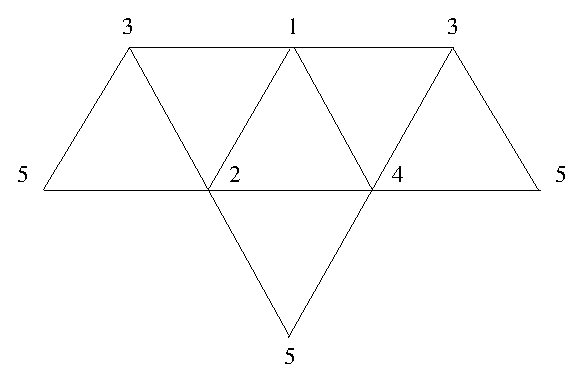
\includegraphics{files/Teardrop}
\caption{triangulation} \end{center} \end{figure}   

The source code: 
\begin{Verbatim}[commandchars=!@|,fontsize=\small,frame=single,label=Example]
  !gapprompt@gap>| !gapinput@M := [ [1,2,3], [1,2,4], [1,3,4], [2,3,5], [2,4,5], [3,4,5] ];;|
  !gapprompt@gap>| !gapinput@iso := rec( 1 := Group( (1,2) ) );;|
  !gapprompt@gap>| !gapinput@mu := [|
  !gapprompt@>| !gapinput@           [ [3], [1,3], [1,2,3], [1,3,4], x -> (1,2) ],|
  !gapprompt@>| !gapinput@           [ [3], [1,3], [1,3,4], [1,2,3], x -> (1,2) ]|
  !gapprompt@>| !gapinput@         ];;|
  !gapprompt@gap>| !gapinput@ot := OrbifoldTriangulation( M, iso, mu, "Teardrop" );|
  <OrbifoldTriangulation "Teardrop" of dimension 2. 6 simplices on 5 vertices wi\
  th Isotropy on 1 vertex and nontrivial mu-maps>
  !gapprompt@gap>| !gapinput@ss := SimplicialSet( ot );|
  <The simplicial set of the orbifold triangulation "Teardrop", computed up to d\
  imension 0 with Length vector [ 6 ]>
  !gapprompt@gap>| !gapinput@R := HomalgRingOfIntegers();|
  Z
  !gapprompt@gap>| !gapinput@c := CreateCoboundaryMatrices( ss, 6, R );;|
  !gapprompt@gap>| !gapinput@C := Cohomology( c, R );|
  ----------------------------------------------->>>>  Z^(1 x 1)
  ----------------------------------------------->>>>  0
  ----------------------------------------------->>>>  Z^(1 x 1)
  ----------------------------------------------->>>>  0
  ----------------------------------------------->>>>  Z/< 2 >
  ----------------------------------------------->>>>  0
  ----------------------------------------------->>>>  Z/< 2 >
  <A graded cohomology object consisting of 7 left modules at degrees
  [ 0 .. 6 ]>
\end{Verbatim}
 This is the Teardrop cohomology. }

 }

   
\chapter{\textcolor{Chapter }{\textsf{SCO} methods and functions}}\label{ch:MandF}
\logpage{[ 4, 0, 0 ]}
\hyperdef{L}{X84058CCC8552F8A9}{}
{
 
\section{\textcolor{Chapter }{Methods and functions for orbifold triangulations}}\logpage{[ 4, 1, 0 ]}
\hyperdef{L}{X822BCAB878B669A5}{}
{
 

\subsection{\textcolor{Chapter }{OrbifoldTriangulation}}
\logpage{[ 4, 1, 1 ]}\nobreak
\hyperdef{L}{X817F45D6780F45F7}{}
{\noindent\textcolor{FuncColor}{$\triangleright$\ \ \texttt{OrbifoldTriangulation({\mdseries\slshape M[, I, mu{\textunderscore}data, info]})\index{OrbifoldTriangulation@\texttt{OrbifoldTriangulation}}
\label{OrbifoldTriangulation}
}\hfill{\scriptsize (function)}}\\
\textbf{\indent Returns:\ }
OrbifoldTriangulation



 The constructor for OrbifoldTriangulations. Needs the list \mbox{\texttt{\mdseries\slshape M}} of maximal simplices, the Isotropy at certain vertices as a record \mbox{\texttt{\mdseries\slshape I}}, and the list \mbox{\texttt{\mdseries\slshape mu{\textunderscore}data}} that encodes the function mu. If only one argument is given, \mbox{\texttt{\mdseries\slshape I}} and \mbox{\texttt{\mdseries\slshape mu{\textunderscore}data}} are supposed to be empty. In case of two arguments, \mbox{\texttt{\mdseries\slshape mu{\textunderscore}data}} is supposed to be empty. If the last argument \mbox{\texttt{\mdseries\slshape info}} is given as a string, it is stored in the info component of the orbifold
triangulation and does not count towards the total number of arguments. 
\begin{Verbatim}[commandchars=!@|,fontsize=\small,frame=single,label=Example]
  !gapprompt@gap>| !gapinput@M := [ [1,2,3], [1,2,4], [1,3,4], [2,3,4] ];;|
  !gapprompt@gap>| !gapinput@S2 := OrbifoldTriangulation( M, "S^2" );|
  <OrbifoldTriangulation "S^2" of dimension 2. 4 simplices on 4 vertices without\
   Isotropy>
  !gapprompt@gap>| !gapinput@I := rec( 1 := Group( (1,2) ) );;|
  !gapprompt@gap>| !gapinput@mu_data := [|
  !gapprompt@>| !gapinput@[ [2], [1,2], [1,2,3], [1,2,4], x->x*(1,2) ],|
  !gapprompt@>| !gapinput@[ [2], [1,2], [1,2,4], [1,2,3], x->x*(1,2) ]|
  !gapprompt@>| !gapinput@];;|
  !gapprompt@gap>| !gapinput@Teardrop := OrbifoldTriangulation( M, I, mu_data, "Teardrop" );|
  <OrbifoldTriangulation "Teardrop" of dimension 2. 4 simplices on 4 vertices wi\
  th Isotropy on 1 vertex and nontrivial mu-maps>
\end{Verbatim}
 }

 

\subsection{\textcolor{Chapter }{Vertices}}
\logpage{[ 4, 1, 2 ]}\nobreak
\hyperdef{L}{X79E4BB4F849AC8A1}{}
{\noindent\textcolor{FuncColor}{$\triangleright$\ \ \texttt{Vertices({\mdseries\slshape ot})\index{Vertices@\texttt{Vertices}}
\label{Vertices}
}\hfill{\scriptsize (method)}}\\
\textbf{\indent Returns:\ }
List \mbox{\texttt{\mdseries\slshape V}}



 This returns the list of vertices \mbox{\texttt{\mdseries\slshape V}} of the orbifold triangulation \mbox{\texttt{\mdseries\slshape ot}}. Should be preferred to the equivalent \texttt{ot!.vertices}. }

 

\subsection{\textcolor{Chapter }{Simplices}}
\logpage{[ 4, 1, 3 ]}\nobreak
\hyperdef{L}{X7AC3235E8044172B}{}
{\noindent\textcolor{FuncColor}{$\triangleright$\ \ \texttt{Simplices({\mdseries\slshape ot})\index{Simplices@\texttt{Simplices}}
\label{Simplices}
}\hfill{\scriptsize (method)}}\\
\textbf{\indent Returns:\ }
List \mbox{\texttt{\mdseries\slshape M}}



 This returns the list of maximal simplices \mbox{\texttt{\mdseries\slshape M}} of the orbifold triangulation \mbox{\texttt{\mdseries\slshape ot}}. Should be preferred to the equivalent \texttt{ot!.max{\textunderscore}simplices}. }

 

\subsection{\textcolor{Chapter }{Isotropy}}
\logpage{[ 4, 1, 4 ]}\nobreak
\hyperdef{L}{X7D9F409380816CB5}{}
{\noindent\textcolor{FuncColor}{$\triangleright$\ \ \texttt{Isotropy({\mdseries\slshape ot})\index{Isotropy@\texttt{Isotropy}}
\label{Isotropy}
}\hfill{\scriptsize (method)}}\\
\textbf{\indent Returns:\ }
Record \mbox{\texttt{\mdseries\slshape I}}



 This returns the isotropy record \mbox{\texttt{\mdseries\slshape I}} of the orbifold triangulation \mbox{\texttt{\mdseries\slshape ot}}. Should be preferred to the equivalent \texttt{ot!.isotropy}. }

 

\subsection{\textcolor{Chapter }{Mu}}
\logpage{[ 4, 1, 5 ]}\nobreak
\hyperdef{L}{X795D2855804A5855}{}
{\noindent\textcolor{FuncColor}{$\triangleright$\ \ \texttt{Mu({\mdseries\slshape ot})\index{Mu@\texttt{Mu}}
\label{Mu}
}\hfill{\scriptsize (method)}}\\
\textbf{\indent Returns:\ }
Function \mbox{\texttt{\mdseries\slshape mu}}



 This returns the function \mbox{\texttt{\mdseries\slshape mu}} of the orbifold triangulation \mbox{\texttt{\mdseries\slshape ot}}. Should be preferred to the equivalent \texttt{ot!.mu}. }

 

\subsection{\textcolor{Chapter }{MuData}}
\logpage{[ 4, 1, 6 ]}\nobreak
\hyperdef{L}{X83926F268523C541}{}
{\noindent\textcolor{FuncColor}{$\triangleright$\ \ \texttt{MuData({\mdseries\slshape ot})\index{MuData@\texttt{MuData}}
\label{MuData}
}\hfill{\scriptsize (method)}}\\
\textbf{\indent Returns:\ }
List \mbox{\texttt{\mdseries\slshape mu{\textunderscore}data}}



 This returns the list \mbox{\texttt{\mdseries\slshape mu{\textunderscore}data}} that encodes the function mu of the orbifold triangulation \mbox{\texttt{\mdseries\slshape ot}}. Should be preferred to the equivalent \texttt{ot!.mu{\textunderscore}data}. }

 

\subsection{\textcolor{Chapter }{InfoString}}
\logpage{[ 4, 1, 7 ]}\nobreak
\hyperdef{L}{X7E845DE47C817088}{}
{\noindent\textcolor{FuncColor}{$\triangleright$\ \ \texttt{InfoString({\mdseries\slshape ot})\index{InfoString@\texttt{InfoString}}
\label{InfoString}
}\hfill{\scriptsize (method)}}\\
\textbf{\indent Returns:\ }
String \mbox{\texttt{\mdseries\slshape info}}



 This return the string \mbox{\texttt{\mdseries\slshape info}} of the orbifold triangulation \mbox{\texttt{\mdseries\slshape ot}}. Should be preferred to the equivalent \texttt{ot!.info}. }

 }

 
\section{\textcolor{Chapter }{Methods and functions for simplicial sets}}\logpage{[ 4, 2, 0 ]}
\hyperdef{L}{X7B0172DD7CD92CD8}{}
{
 

\subsection{\textcolor{Chapter }{SimplicialSet (constructor)}}
\logpage{[ 4, 2, 1 ]}\nobreak
\hyperdef{L}{X7DD68A0E7E3A4A51}{}
{\noindent\textcolor{FuncColor}{$\triangleright$\ \ \texttt{SimplicialSet({\mdseries\slshape ot})\index{SimplicialSet@\texttt{SimplicialSet}!constructor}
\label{SimplicialSet:constructor}
}\hfill{\scriptsize (method)}}\\
\textbf{\indent Returns:\ }
SimplicialSet



 The constructor for simplicial sets based on an orbifold triangulation \mbox{\texttt{\mdseries\slshape ot}}. This just sets up the object without any computations. These can be
triggered later, either explicitly or by \texttt{SimplicialSet} (\ref{SimplicialSet:data access}). 
\begin{Verbatim}[commandchars=!@|,fontsize=\small,frame=single,label=Example]
  !gapprompt@gap>| !gapinput@Teardrop;|
  <OrbifoldTriangulation "Teardrop" of dimension 2. 4 simplices on 4 vertices wi\
  th Isotropy on 1 vertex and nontrivial mu-maps>
  !gapprompt@gap>| !gapinput@S := SimplicialSet( Teardrop );|
  <The simplicial set of the orbifold triangulation "Teardrop", computed up to d\
  imension 0 with Length vector [ 4 ]>
\end{Verbatim}
 }

 

\subsection{\textcolor{Chapter }{SimplicialSet (data access)}}
\logpage{[ 4, 2, 2 ]}\nobreak
\hyperdef{L}{X7DC060057E853275}{}
{\noindent\textcolor{FuncColor}{$\triangleright$\ \ \texttt{SimplicialSet({\mdseries\slshape S, i})\index{SimplicialSet@\texttt{SimplicialSet}!data access}
\label{SimplicialSet:data access}
}\hfill{\scriptsize (method)}}\\
\textbf{\indent Returns:\ }
List \mbox{\texttt{\mdseries\slshape S}}{\textunderscore}\mbox{\texttt{\mdseries\slshape i}}



 This returns the components of dimension \mbox{\texttt{\mdseries\slshape i}} of the simplicial set \mbox{\texttt{\mdseries\slshape S}}. Should be used to access existing data instead of using \texttt{S!.simplicial{\textunderscore}set[ i + 1 ]}, as it has the additional side effect of computing \mbox{\texttt{\mdseries\slshape S}} up to dimension \mbox{\texttt{\mdseries\slshape i}}, thus always returning the desired result. 
\begin{Verbatim}[commandchars=@|A,fontsize=\small,frame=single,label=Example]
  @gapprompt|gap>A @gapinput|S := SimplicialSet( Teardrop );A
  <The simplicial set of the orbifold triangulation "Teardrop", computed up to d\
  imension 0 with Length vector [ 4 ]>
  @gapprompt|gap>A @gapinput|S!.simplicial_set[1];A
  [ [ [ 1, 2, 3 ] ], [ [ 1, 2, 4 ] ], [ [ 1, 3, 4 ] ], [ [ 2, 3, 4 ] ] ]
  @gapprompt|gap>A @gapinput|S!.simplicial_set[2];;A
  Error, List Element: <list>[2] must have an assigned value
  @gapprompt|gap>A @gapinput|SimplicialSet( S, 0 );A
  [ [ [ 1, 2, 3 ] ], [ [ 1, 2, 4 ] ], [ [ 1, 3, 4 ] ], [ [ 2, 3, 4 ] ] ]
  @gapprompt|gap>A @gapinput|SimplicialSet( S, 1 );;A
  @gapprompt|gap>A @gapinput|S;A
  <The simplicial set of the orbifold triangulation "Teardrop", computed up to d\
  imension 1 with Length vector [ 4, 12 ]>
\end{Verbatim}
 }

 

\subsection{\textcolor{Chapter }{ComputeNextDimension}}
\logpage{[ 4, 2, 3 ]}\nobreak
\hyperdef{L}{X80091ADD7F0D80F2}{}
{\noindent\textcolor{FuncColor}{$\triangleright$\ \ \texttt{ComputeNextDimension({\mdseries\slshape S})\index{ComputeNextDimension@\texttt{ComputeNextDimension}}
\label{ComputeNextDimension}
}\hfill{\scriptsize (method)}}\\
\textbf{\indent Returns:\ }
\mbox{\texttt{\mdseries\slshape S}}



 This computes the component of the next dimension of the simplicial set \mbox{\texttt{\mdseries\slshape S}}. \mbox{\texttt{\mdseries\slshape S}} is extended as a side effect. 
\begin{Verbatim}[commandchars=!@|,fontsize=\small,frame=single,label=Example]
  !gapprompt@gap>| !gapinput@S;|
  <The simplicial set of the orbifold triangulation "Teardrop", computed up to d\
  imension 1 with Length vector [ 4, 12 ]>
  !gapprompt@gap>| !gapinput@ComputeNextDimension( S );|
  <The simplicial set of the orbifold triangulation "Teardrop", computed up to d\
  imension 2 with Length vector [ 4, 12, 22 ]>
\end{Verbatim}
 }

 

\subsection{\textcolor{Chapter }{Extend}}
\logpage{[ 4, 2, 4 ]}\nobreak
\hyperdef{L}{X7BAB245A8009088D}{}
{\noindent\textcolor{FuncColor}{$\triangleright$\ \ \texttt{Extend({\mdseries\slshape S, i})\index{Extend@\texttt{Extend}}
\label{Extend}
}\hfill{\scriptsize (method)}}\\
\textbf{\indent Returns:\ }
\mbox{\texttt{\mdseries\slshape S}}



 This computes the components of the simplicial set \mbox{\texttt{\mdseries\slshape S}} up to dimension \mbox{\texttt{\mdseries\slshape i}}. \mbox{\texttt{\mdseries\slshape S}} is extended as a side effect. This method is equivalent to calling \texttt{ComputeNextDimension} (\ref{ComputeNextDimension}) the appropriate number of times. 
\begin{Verbatim}[commandchars=!@|,fontsize=\small,frame=single,label=Example]
  !gapprompt@gap>| !gapinput@S;|
  <The simplicial set of the orbifold triangulation "Teardrop", computed up to d\
  imension 2 with Length vector [ 4, 12, 22 ]>
  !gapprompt@gap>| !gapinput@Extend( S, 5 );|
  <The simplicial set of the orbifold triangulation "Teardrop", computed up to d\
  imension 5 with Length vector [ 4, 12, 22, 33, 51, 73 ]>
\end{Verbatim}
 }

 }

 
\section{\textcolor{Chapter }{Methods and functions for matrix creation and computation}}\logpage{[ 4, 3, 0 ]}
\hyperdef{L}{X87335B4B8437DA4B}{}
{
 

\subsection{\textcolor{Chapter }{BoundaryOperator}}
\logpage{[ 4, 3, 1 ]}\nobreak
\hyperdef{L}{X7F28FA7B83B681E8}{}
{\noindent\textcolor{FuncColor}{$\triangleright$\ \ \texttt{BoundaryOperator({\mdseries\slshape i, L, mu})\index{BoundaryOperator@\texttt{BoundaryOperator}}
\label{BoundaryOperator}
}\hfill{\scriptsize (function)}}\\
\textbf{\indent Returns:\ }
List B



 This returns the \mbox{\texttt{\mdseries\slshape i}}th boundary of \mbox{\texttt{\mdseries\slshape L}}, which has to be an element of a simplicial set. \mbox{\texttt{\mdseries\slshape mu}} is the function $\mu$ that has to be taken into account when computing orbifold boundaries. This
function is used for matrix creation, there should not be much reason for
calling it independently. }

 

\subsection{\textcolor{Chapter }{CreateBoundaryMatrices}}
\logpage{[ 4, 3, 2 ]}\nobreak
\hyperdef{L}{X80C3C6867CE9FE3E}{}
{\noindent\textcolor{FuncColor}{$\triangleright$\ \ \texttt{CreateBoundaryMatrices({\mdseries\slshape S, d, R})\index{CreateBoundaryMatrices@\texttt{CreateBoundaryMatrices}}
\label{CreateBoundaryMatrices}
}\hfill{\scriptsize (method)}}\\
\textbf{\indent Returns:\ }
List \mbox{\texttt{\mdseries\slshape M}}



 This returns the list \mbox{\texttt{\mdseries\slshape M}} of homalg matrices over the homalg ring \mbox{\texttt{\mdseries\slshape R}} up to dimension \mbox{\texttt{\mdseries\slshape d}}, corresponding to the boundary matrices induced by the simplicial set \mbox{\texttt{\mdseries\slshape S}}. If \mbox{\texttt{\mdseries\slshape d}} is not given, the current dimension of \mbox{\texttt{\mdseries\slshape S}} is used. 
\begin{Verbatim}[commandchars=!@|,fontsize=\small,frame=single,label=Example]
  !gapprompt@gap>| !gapinput@S := SimplicialSet( Teardrop );|
  <The simplicial set of the orbifold triangulation "Teardrop", computed up to d\
  imension 0 with Length vector [ 4 ]>
  !gapprompt@gap>| !gapinput@M := CreateBoundaryMatrices( S, 4, HomalgRingOfIntegers() );;|
  !gapprompt@gap>| !gapinput@S;|
  <The simplicial set of the orbifold triangulation "Teardrop", computed up to d\
  imension 5 with Length vector [ 4, 12, 22, 33, 51, 73 ]>
\end{Verbatim}
 }

 

\subsection{\textcolor{Chapter }{Homology}}
\logpage{[ 4, 3, 3 ]}\nobreak
\hyperdef{L}{X85A9D5CB8605329C}{}
{\noindent\textcolor{FuncColor}{$\triangleright$\ \ \texttt{Homology({\mdseries\slshape M[, R]})\index{Homology@\texttt{Homology}}
\label{Homology}
}\hfill{\scriptsize (method)}}\\
\textbf{\indent Returns:\ }
a \textsf{homalg} complex



 This returns the homology complex of a list \mbox{\texttt{\mdseries\slshape M}} of \textsf{homalg} matrices over the \textsf{homalg} ring \mbox{\texttt{\mdseries\slshape R}}. 
\begin{Verbatim}[commandchars=!@|,fontsize=\small,frame=single,label=Example]
  !gapprompt@gap>| !gapinput@S := SimplicialSet( Teardrop );|
  <The simplicial set of the orbifold triangulation "Teardrop", computed up to d\
  imension 0 with Length vector [ 4 ]>
  !gapprompt@gap>| !gapinput@R := HomalgRingOfIntegers();|
  Z
  !gapprompt@gap>| !gapinput@M := CreateBoundaryMatrices( S, 4, R );;|
  !gapprompt@gap>| !gapinput@Homology( M, R );|
  ----------------------------------------------->>>>  Z^(1 x 1)
  ----------------------------------------------->>>>  0
  ----------------------------------------------->>>>  Z^(1 x 1)
  ----------------------------------------------->>>>  Z/< 2 >
  ----------------------------------------------->>>>  0
  <A graded homology object consisting of 5 left modules at degrees [ 0 .. 4 ]>
\end{Verbatim}
 }

 

\subsection{\textcolor{Chapter }{CreateCoboundaryMatrices}}
\logpage{[ 4, 3, 4 ]}\nobreak
\hyperdef{L}{X8320B03E7FEB2BA8}{}
{\noindent\textcolor{FuncColor}{$\triangleright$\ \ \texttt{CreateCoboundaryMatrices({\mdseries\slshape S[, d], R})\index{CreateCoboundaryMatrices@\texttt{CreateCoboundaryMatrices}}
\label{CreateCoboundaryMatrices}
}\hfill{\scriptsize (method)}}\\
\textbf{\indent Returns:\ }
List \mbox{\texttt{\mdseries\slshape M}}



 This returns the list \mbox{\texttt{\mdseries\slshape M}} of homalg matrices over the homalg ring \mbox{\texttt{\mdseries\slshape R}} up to dimension \mbox{\texttt{\mdseries\slshape d}}, corresponding to the coboundary matrices induced by the simplicial set \mbox{\texttt{\mdseries\slshape S}}. If \mbox{\texttt{\mdseries\slshape d}} is not given, the current dimension of \mbox{\texttt{\mdseries\slshape S}} is used. 
\begin{Verbatim}[commandchars=!@|,fontsize=\small,frame=single,label=Example]
  !gapprompt@gap>| !gapinput@S := SimplicialSet( Teardrop );|
  <The simplicial set of the orbifold triangulation "Teardrop", computed up to d\
  imension 0 with Length vector [ 4 ]>
  !gapprompt@gap>| !gapinput@M := CreateCoboundaryMatrices( S, 4, HomalgRingOfIntegers() );;|
  !gapprompt@gap>| !gapinput@S;|
  <The simplicial set of the orbifold triangulation "Teardrop", computed up to d\
  imension 5 with Length vector [ 4, 12, 22, 33, 51, 73 ]>
\end{Verbatim}
 }

 

\subsection{\textcolor{Chapter }{Cohomology}}
\logpage{[ 4, 3, 5 ]}\nobreak
\hyperdef{L}{X84CFC57B7E9CCCF7}{}
{\noindent\textcolor{FuncColor}{$\triangleright$\ \ \texttt{Cohomology({\mdseries\slshape M[, R]})\index{Cohomology@\texttt{Cohomology}}
\label{Cohomology}
}\hfill{\scriptsize (method)}}\\
\textbf{\indent Returns:\ }
a \textsf{homalg} complex



 This returns the cohomology complex of a list \mbox{\texttt{\mdseries\slshape M}} of \textsf{homalg} matrices over the \textsf{homalg} ring \mbox{\texttt{\mdseries\slshape R}}. 
\begin{Verbatim}[commandchars=!@|,fontsize=\small,frame=single,label=Example]
  !gapprompt@gap>| !gapinput@S := SimplicialSet( Teardrop );|
  <The simplicial set of the orbifold triangulation "Teardrop", computed up to d\
  imension 0 with Length vector [ 4 ]>
  !gapprompt@gap>| !gapinput@R := HomalgRingOfIntegers();|
  Z
  !gapprompt@gap>| !gapinput@M := CreateCoboundaryMatrices( S, 4, R );;|
  !gapprompt@gap>| !gapinput@Cohomology( M, R );|
  ----------------------------------------------->>>>  Z^(1 x 1)
  ----------------------------------------------->>>>  0
  ----------------------------------------------->>>>  Z^(1 x 1)
  ----------------------------------------------->>>>  0
  ----------------------------------------------->>>>  Z/< 2 >
  <A graded cohomology object consisting of 5 left modules at degrees
  [ 0 .. 4 ]>
\end{Verbatim}
 }

 

\subsection{\textcolor{Chapter }{SCO{\textunderscore}Examples}}
\logpage{[ 4, 3, 6 ]}\nobreak
\hyperdef{L}{X85874A8979FF9E82}{}
{\noindent\textcolor{FuncColor}{$\triangleright$\ \ \texttt{SCO{\textunderscore}Examples({\mdseries\slshape })\index{SCOExamples@\texttt{SCO{\textunderscore}Examples}}
\label{SCOExamples}
}\hfill{\scriptsize (function)}}\\
\textbf{\indent Returns:\ }
nothing



 This is just an easy way to call the script \texttt{examples.g}, which is located in \texttt{gap/pkg/SCO/examples/}. 
\begin{Verbatim}[commandchars=!|B,fontsize=\small,frame=single,label=Example]
  !gapprompt|gap>B !gapinput|SCO_Examples();B
  @@@@@@@@ SCO @@@@@@@@
  
  Select base ring:
   1) Integers (default)
   2) Rationals
   3) Z/nZ
  :1
  
  Select Computer Algebra System:
   1) GAP (default)
   2) External GAP
   3) MAGMA
   4) Maple
   5) Sage
  :3
  ---------------------------------------------------------------
  Magma V2.14-14    Tue Aug 19 2008 08:36:19 on evariste [Seed = 1054613462]
  Type ? for help.  Type <Ctrl>-D to quit.
  ----------------------------------------------------------------
  
  
  Select Method:
   1) Full syzygy computation (default)
   2) matrix creation and rank computation only
  :1
  
  Select orbifold (default="C2")
  :Torus
    
  Select mode:
   1) Cohomology (default)
   2) Homology
  :1
  
  Select dimension (default = 4)
  :4
  Creating the coboundary matrices ...
  Starting cohomology computation ...
  ----------------------------------------------->>>>  Z^(1 x 1)
  ----------------------------------------------->>>>  Z^(1 x 2)
  ----------------------------------------------->>>>  Z^(1 x 1)
  ----------------------------------------------->>>>  0
  ----------------------------------------------->>>>  0    
\end{Verbatim}
 }

 }

 }

 

\appendix


\chapter{\textcolor{Chapter }{An Overview of the \textsf{SCO} package source code}}\label{FileOverview}
\logpage{[ "A", 0, 0 ]}
\hyperdef{L}{X87781B6F824EC8DE}{}
{
  \begin{center}
\begin{tabular}{l|l}Filename&
Content\\
\hline
OrbifoldTriangulation.gi&
Definitions and methods for orbifold triangulations\\
SimplicialSet.gi&
Definitions and methods for simplicial sets\\
Matrices.gi&
Methods for (Co-)homology matrix creation\\
SCO.gi&
(Co-)homology computations and \texttt{SCO{\textunderscore}Examples} (\ref{SCOExamples})\\
\end{tabular}\\[2mm]
\textbf{Table: }\emph{The \textsf{SCO} package files.}\end{center}

 }

\def\bibname{References\logpage{[ "Bib", 0, 0 ]}
\hyperdef{L}{X7A6F98FD85F02BFE}{}
}

\bibliographystyle{alpha}
\bibliography{SCOBib.xml}

\addcontentsline{toc}{chapter}{References}

\def\indexname{Index\logpage{[ "Ind", 0, 0 ]}
\hyperdef{L}{X83A0356F839C696F}{}
}

\cleardoublepage
\phantomsection
\addcontentsline{toc}{chapter}{Index}


\printindex

\newpage
\immediate\write\pagenrlog{["End"], \arabic{page}];}
\immediate\closeout\pagenrlog
\end{document}
